\subsection{Excercise TestCarRentalCLI}
\label{sec:exercise_test_car_rental_cli}
This task is about testing the CarRentalCLI application, to be more specific, the \texttt{RentACar} function.

The \texttt{RentACar} function is located in the \texttt{operations} package in the \hfill \linebreak \texttt{RentACarOperation.go} file.
It takes the rentalID, the customerID, the carID, and start and endDate as arguments and returns a String and an error.

During its execution, it checks the given arguments for validity and checks the pre-condition.
If the pre-condition is met, the function creates a new rental and adds it to the repository.
If one of the checks fails, or an error occurs during runtime, the function returns an error.

After successfully creating the new rental by calling the \texttt{repository.CreateRental()} function, a string indicating the success concatenated with the rental ID is returned.

\texttt{RentACarOperation\_text.go} contains the tests and the according data for the testing environments to test the \texttt{RentACar} function.
The goal of the following tasks is to derive test cases from given OCL constraints, analyze the test structure, add test data, implement and finally run the tests.

\subsubsection*{Derive Test Cases}
For the sake of simplicity, assume that a correct car called \texttt{correctCar} and a customer called \texttt{correctCustomer} are provided.
In the cases where the date is correct assume the date \texttt{startDate} and \texttt{endDate} represent correct dates.
In this example assume the start Date to be 01.01.2000 and the end Date to be 02.02.2000.

\autoref{lstlisting:rental_test_cases} defines positive and negative test cases for the \texttt{NewRental} function.
\begin{lstlisting}[
style=kit-cm,
language=Golang,
caption={Test Cases for the Rental Context},
label={lstlisting:rental_test_cases},
]
// Constraint 1: self.ID -> notEmpty()
NewRental("", startDate, endDate, correctCar, correctCustomer) // negative test case
NewRental("Rental1", startDate, endDate, correctCar, correctCustomer) // positive test case

// Constraint 2: self.startDate -> notEmty()
NewRental("Rental2", date{}, endDate, correctCar, correctCustomer) // negative test case
NewRental("Rental2", startDate, endDate, correctCar, correctCustomer) // positive test case

// Constraint 3: self.endDate -> notEmty()
NewRental("Rental3", startDate, date{}, correctCar, correctCustomer) // negative test case
NewRental("Rental3", startDate, endDate, correctCar, correctCustomer) // positive test case

// Constraint 4: self.startDate < self.endDate
NewRental("Rental4", endDate, startDate, correctCar, correctCustomer) // negative test case
NewRental("Rental4", startDate, endDate, correctCar, correctCustomer) // positive test case

// Constraint 5: self.car -> notEmpty()
NewRental("Rental5", startDate, endDate, car{}, correctCustomer) // negative test case
NewRental("Rental5", startDate, endDate, correctCar, correctCustomer) // positive test case

// Constraint 6: self.customer -> notEmpty()
NewRental("Rental6", startDate, endDate, correctCar, customer{}) // negative test case
NewRental("Rental6", startDate, endDate, correctCar, correctCustomer) // positive test case
\end{lstlisting}
  
This paragraph designs positive and negative test cases for the \texttt{rentACar\(\)} function.
This function takes the rental ID, start and end date, the car, and the customer as arguments.
If the function is executed correctly it will return the new rental.
As specified at the beginning of the section, startDate, endDate, correctCar, and correctCustomer represent the correct parameters.

\begin{lstlisting}[
style=kit-cm,
language=Golang,
caption={Test Cases for the Customer Context},
label={lstlisting:customer_test_cases},
]
// Constraint 1: pre: self.rentalID -> not exists
rentACar("Rental1", startDate, endDate, correctCar, correctCustomer)
rentACar("Rental1", startDate, endDate, correctCar, correctCustomer) // negative test case due to function executing twice
rentACar("Rental2", startDate, endDate, correctCar, correctCustomer) // positive test case

// Constraint 2: and Rental.allInstances() -> 
//  forAll(r: Rental | r.car = self.car implies(self.endDate < r.endDate or r.Endate > self.startDate))
rentACar("Rental3", startDate, endDate, correctCar, correctCustomer)
rentACar("Rental4", startDate', endDate, correctCar, correctCustomer') // negative test case due to overlapping dates for the same car
rentACar("Rental5", startDate', endDate', correctCar, correctCustomer') // positive test case 

// Constraint 3: post: self.rentals -> includes(rental)
rentACar("Rental6", startDate, endDate, correctCar, correctCustomer) // positive test case
rentACar("Rental7", date{}, endDate, correctCar, correctCustomer) // negative test case => due to constraint 2, the element will not be created and therefore will not appear in the list

\end{lstlisting}

\subsubsection*{Analyze Test Structure}
% Structure description of the test file and mock-repository
The MockCarRepository acts similarly to the actual CarRepository.
It implements the CarRentalRepositoryInterface and provides the appropriate functions.
Furthermore, it also implements the lists of the models \texttt{Rental}, \texttt{Car}, and \texttt{Customer}.
However, there is no constructor and no manipulation of yaml files.
All data manipulations are done in the memory of the mock repository.
Therefore the mock-repository only imports the used models.

The test file \texttt{RentACarOperation\_test.go} implements the tests for the \texttt{RentACar} function.
It creates the testing environment by implementing the constructor of the mock repository and populating it with test data.
After the setup, the executable tests are implemented.

% Structure description of the test function TestCarRentalOperations_RentACar
The implementation of the tests happens in the \texttt{TestCarRentalOperations\_RentACar} function.
The \texttt{fields} struct defines the repository used in each test and therefore the test environment.
After that, the \texttt{args} struct defines the arguments needed for the \texttt{RentACar} function.
Now, the test cases are implemented containing the following values:
\begin{itemize}
      \item fields: The repository used in the test as specified above
      \item name: The name of the test
      \item args: The arguments for the \texttt{RentACar} function as specified above
      \item want: The expected return value of the \texttt{RentACar} function, in this case a String 
      \item wantErr: True, if an error is expected, false otherwise. 
            This allows the implementation of negative test cases without the tests failing.
\end{itemize}

% Differences between the mock and the normal repository
The following differences occur between the mock and the normal repository:
\begin{itemize}
      \item The mock repository does not implement a constructor
      \item The mock repository does not manipulate any yaml files, everything is done in the mock repository's lists.
      \item The mock repository only imports the models used in the tests.
      \item The mock repository is only used for testing while the normal repository is used in the application.
      \item The mock repository is located in the same package as the test file (operations), while the normal repository is located in the infrastructure package.
\end{itemize}

However, there are still some similarities:
\begin{itemize}
      \item Both repositories implement the CarRentalRepositoryInterface and therefore provide the same functions.
      \item The provided functionalities are somewhat similar besides the differences mentioned above.
      \item Both repositories are addressed via an operations object representing the repository
\end{itemize}

% Why is a mocked repository required?
Now, why is a mocked repository required?
First of all, the mock repository is required to test the functionality of the \texttt{RentACar} function.
This could also be done with the normal repository, however, this would require the manipulation of the yaml files, which raises the following problems:
\begin{itemize}
      \item Test data and actual application data are mixed up
      \item The test data is not reset after the test, which could lead to problems in the next test
      \item The test data needs to be cleaned up after the test, which is not necessary with the mock repository
      \item By creating a certain testing environment, the testing data can be manipulated to test the wanted scenarios
\end{itemize}

Further benefits and the actual usage and implementation of both the normal and the mock repository are further explained in \autoref{sec:go_repositories}.
As shown all tests pass besides the first test.
This is due to the given testing environment.
The rental is already created therefore an error will occur and the test will fail.

\subsubsection*{Add Test Data}
As mentioned above, \texttt{RentACarOperation\_test.go} implements the tests for the \texttt{RentACar} function.

The function \texttt{SetupMockCarRentalRepository()} implements the constructor of the mock repository.
It takes no arguments and returns a MockCarRentalRepository.

The function creates arrays of customers, cars and rentals.
These arrays are then used to initialize the mock repository.
The mock repository is then returned.

To populate an array, it needs to be filled with the according structs as specified in the model package.
The structs are initialized in the array.
An example of the initialization of the customer's array is shown in \autoref{lstlisting:customers_array}.

\begin{lstlisting}[
style=kit-cm,
language=Golang,
caption={Initialization Example of the Customers Array},
label={lstlisting:customers_array},
]
customers := []model.Customer{{
      ID:   "Cus1",
      Name: "Max",
}, {
      ID:   "Cus2",
      Name: "Bob",
}, {
      ID:   "Cus3",
      Name: "Simon",
}}
\end{lstlisting}

If a value is referenced in another struct, the reference is set to the according struct in the different array.
During the initialization of the rentals array, this occurs, for example, as shown in \autoref{lstlisting:rentals_array}.

\begin{lstlisting}[
style=kit-cm,
language=Golang,
caption={Code Snippet of Initializing the Rentals Array},
label={lstlisting:rentals_array},
]
rentals := []model.Rental{{
ID: "Rental1",
StartDate: model.Date{
      Day:   1,
      Month: 3,
      Year:  2000,
},
EndDate: model.Date{
      Day:   15,
      Month: 3,
      Year:  2000,
},
Car:      cars[0],
Customer: customers[0],
}, {
ID: "Rental2",
StartDate: model.Date{
      Day:   3,
      Month: 2,
      Year:  2000,
},
EndDate: model.Date{
      Day:   5,
      Month: 2,
      Year:  2000,
},
Car:      cars[1],
Customer: customers[1],
},
...
}
\end{lstlisting}

\subsubsection*{Implement Test Cases}
The tests are implemented in the \texttt{TestCarRentalOperations\_RentACar(t \*testing.T)} function.
The function takes a testing object as an argument and returns nothing.

The function starts by defining the fields and args structs.
The field struct defines the repository used in each test and therefore the test environment.
The args struct defines the arguments needed for the \texttt{RentACar} function - The rental ID, the customerID, the carID, the start and end date.

After that, the test cases are implemented in the \texttt{tests} array.
A test case consists of the test name, the fields, args, the expected return string and a boolean indicating if an error is expected, called \texttt{wantErr}.
Just like in \autoref{lstlisting:customers_array} the arrays are initialized with the according structs.

This task is about implementing the test cases specified in \autoref{lstlisting:rental_test_cases} in the \hfill \linebreak \texttt{TestCarRentalOperations\_RentACar}'s \texttt{tests} array.
A code snippet of two fully implemented test cases is shown in \autoref{lstlisting:test_case_implementation}.

\texttt{NegativeRentalsOverlap} is an example of a negative test case.
A similar rental renting the same car has already been created.
Since the dates of both rentals overlap, a new rental cannot be created.

\begin{lstlisting}[
      style=kit-cm,
      language=Golang,
      caption={Code Snippet of the Test Case Implementation},
      label={lstlisting:test_case_implementation},
]
tests := []struct {
      name    string
      fields  fields
      args    args
      want    string
      wantErr bool
}{
      
		{
			name:   "NegativeRentalsOverlap",
			fields: fields{repository: SetupMockCarRentalRepository()},
			args: args{
				rentalID:   "Rental6",
				customerID: "Cus4",
				carID:      "Car5",
				startDate: model.Date{
					Day:   6,
					Month: 2,
					Year:  2000,
				},
				endDate: model.Date{
					Day:   12,
					Month: 3,
					Year:  2000,
				},
			},
			want:    "",
			wantErr: true,
		},
      ... //Further test cases
}
\end{lstlisting}

\subsection*{Run Tests}
Tests can be started by using Visual Studio Code's graphical features.
By clicking on the starting button next to the function definition of \texttt{TestCarRentalOperations\_RentACar()}, the function is executed as a test.

VSC offers a "Test Result" bar in the terminal panel, visualizing the tests executed and also specifying the start time, runtime and time of completion.
This output is shown in \autoref{fig:carRentalCLI_testingConsoleOutput}.

Right next to this bar, a graphical representation of the tests is shown.
This is shown in \autoref{fig:carRentalCLI_testingGraphicalOutput}.
The green checkmarks indicate successful tests, while the red crosses indicate failed tests.
Single tests can be rerun if wanted by clicking on the according test.
This allows the developer to quickly rerun tests offering a more efficient debugging process.

As mentioned above \autoref{fig:carRentalCLI_testingConsoleOutput} and \autoref{fig:carRentalCLI_testingGraphicalOutput} show the testing results of the tests specified in the previous subtasks.

The first test fails, since it is designed to be a positive test case, however, the rental is already created.
This leads to an error during execution and the test fails due to the \texttt{wantErr} attribute being set to \texttt{false}.

The other tests succeed since they are designed to be negative test cases therefore expecting an error during execution.

\begin{figure}
      \centering
      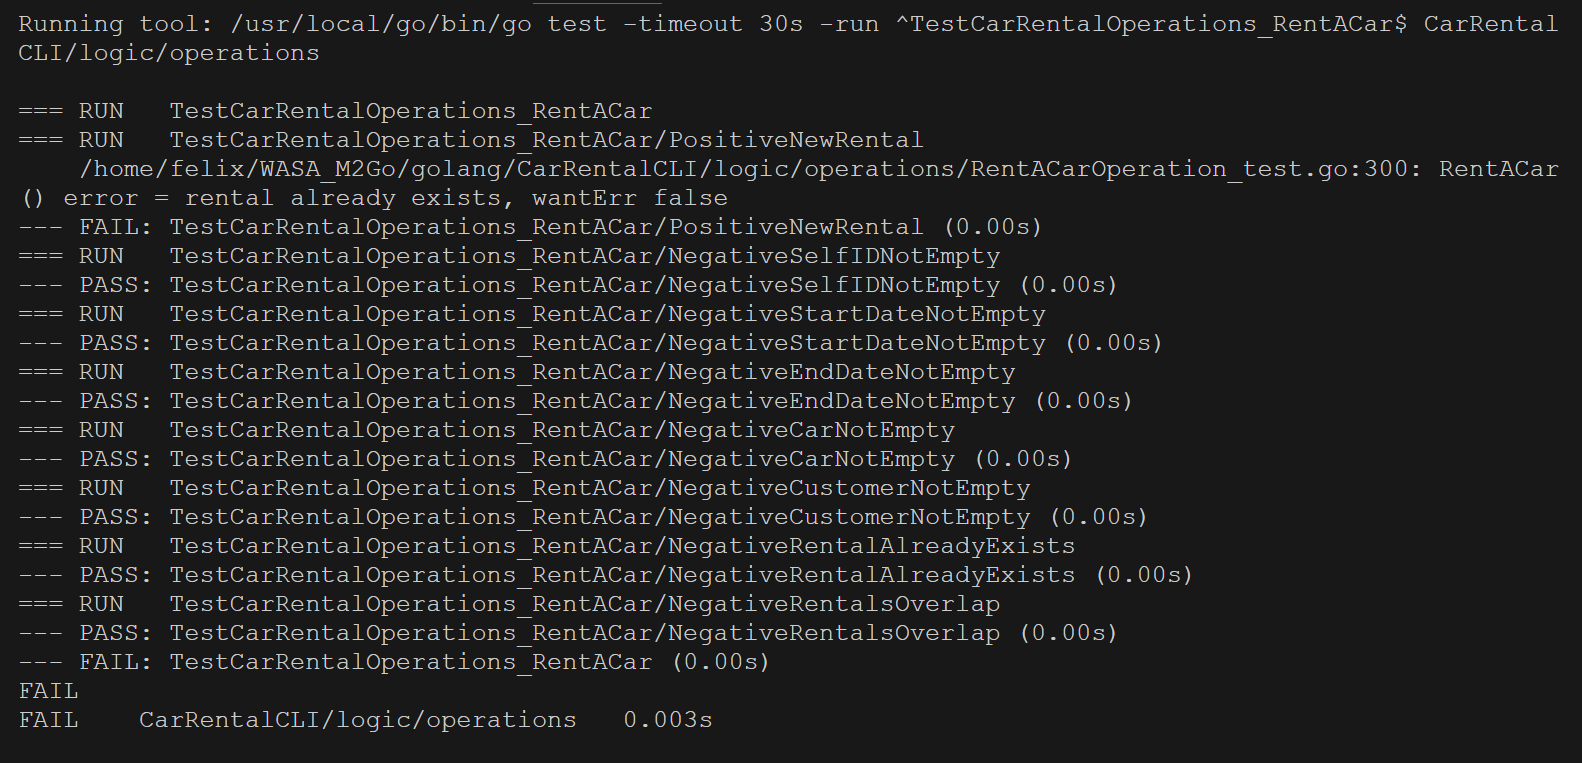
\includegraphics[width=0.8\textwidth]{figures/goLang/carRental/carRentalCLI/carRentalCLI_testingConsoleOutput.png}
      \caption{Console Output of the RentACar Tests}
      \label{fig:carRentalCLI_testingConsoleOutput}
\end{figure}
\begin{figure}
      \centering
      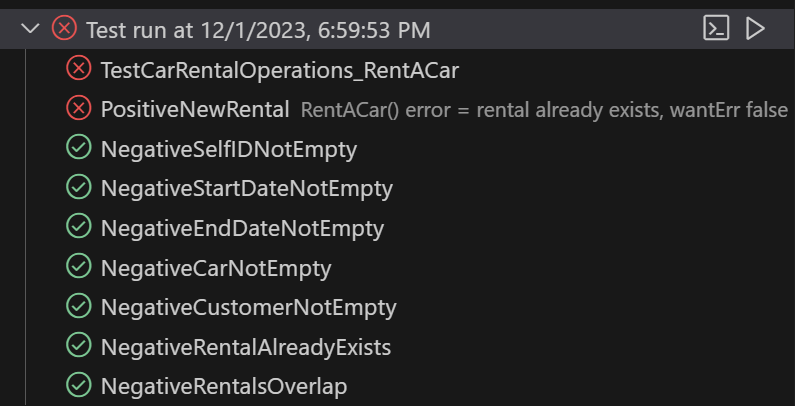
\includegraphics[width=0.8\textwidth]{figures/goLang/carRental/carRentalCLI/carRentalCLI_testingGraphicalOutput.png}
      \caption{Graphical Output of the RentACar Tests}
      \label{fig:carRentalCLI_testingGraphicalOutput}
\end{figure}



